\documentclass[a4paper,12pt]{report}

\usepackage{unipi}

\course{Computer Engineering}
\class{Intelligent Systems}
\title{Using PPG signals in intelligent systems}
\subtitle{Course Project}
\authors{Niccolò Scatena}
\academicyear{2021/2022}

\includeonly{%
	abstract,
	chapters/intro,
	chapters/dataset,
	chapters/ecg,
	chapters/activity,
	chapters/fuzzy,
	chapters/cnn,
	chapters/rnn,
}

\begin{document}

\maketitle
\begin{abstract}
	This project has been developed for the course of \theclass{}
	(\thecourse, \theinstitute). The aim of this project is to design and
	optimize different intelligent systems (neural networks and fuzzy
	inference systems) in order to estimate or predict electrocardiogram
	(ECG) values from signals obtained via photoplethsysmography (PPG)
	sensors.
\end{abstract}


\microtypesetup{protrusion=false}
\tableofcontents
\microtypesetup{protrusion=true}

\chapter{Introduction}\label{ch:intro}

The aim of the project is to design and develop different intelligent systems
that take as input some PPG signals collected from 22 subjects while they were
performing different activities (sit, walk and run).

This chapter describes the organization of the project's MATLAB source code, in
order to allow the reader to easily navigate through the code and understand
the structure of the project.

\section{Organization of the project}\label{sec:organization}

% TODO project files

% TODO directories & files

\subsection{Stages and pipelines}\label{subsec:stagespipeline}


\section{Notes on executing the scripts}\label{sec:execnotes}


\chapter{Dataset}\label{ch:dataset}

This chapter describes the preliminary work done on the dataset in order to
prepare it to train and test the intelligent systems described in the next
chapters.

The first stages of most pipelines used in this project are the following:
\begin{description}
\item[preparedata] This stage loads the data from the CSV files and builds a
	MATLAB structure with a field for each subject. Each field is a
	structure itself with a field for each activity containing a timetable
	with a column for each signal (including the ECG signal).
\item[fixdata] This stage checks that each timetable built in the previous
	stage does not contain any large ``hole'' (a long period of time
	without data). If such a hole is found, the timetable is splitted into
	2 timetables, creating a new subject. The resulting MATLAB structure
	has the same fields as before. In particular, this stage is used to fix
	the data of subject \texttt{s1} during the activity \texttt{sit} which
	has a large 1 hour hole in the middle of the data. A new subject
	(\texttt{s23}) is created with the only activity \texttt{sit}. From
	execution output:
	\begin{verbatim}
	*** STAGE fixdata ***
	Subject 1, activity sit: 2 DIFFERENT time deltas
	(largest: 01:03:06.917). Some are too large.
	Splitting...1-140932...140933-254026(->s23)...done!
	\end{verbatim}
\item[augmentdata] This stage performs data augmentation via random
	subsampling, as explained in \secref{sec:augmentdata}.
\item[getfeatures] This stage simply returns a list of features to extract. See
	\secref{subsec:getfeaturesstage}.
\item[extractfeatures] This stage extracts all the features specified by the
	previous stage (\texttt{getfeatures}) from the augmented dataset. This
	stage is described in details in \secref{subsec:extractfeaturesstage}.
\item[extracttargets] Extract the targets (ECG mean, standard deviation and
	activity) from the augmented dataset, as described in
	\secref{subsec:extracttargetsstage}.
\end{description}

\section{Data augmentation}\label{sec:augmentdata}

The provided data is not sufficient to train the intelligent systems required
by the Project Specifications: there are only 22 subjects recorded during 3
different activities, so there are only a total of 66 recordings available
(plus one more, after the \texttt{fixdata} stage).

Data augmentation is performed by the \texttt{augmentdata} stage. I considered
several methods for data augmentation:
\begin{enumerate}
\item Data augmentation by \standout{adding some noise or distorsions} to
	available signals.
\item \emph{Feature} augmentation using a \standout{variational autoencoder}.
\item Data augmentation via a \standout{(Conditional) (Wasserstein) Generative
	Adversarial Network} (CW-GAN).
\item Data augmentation via \standout{random subsampling}.
\end{enumerate}

The first method was discarded because I need to extract several dozen samples
from each recording to have a fair amount of data for the purposes of this
project: the dataset after the augmentation would be composed of different
groups of similar samples, and the intelligent systems would probably learn to
predict the group of the sample instead of generalizing, leading to
overfitting.

The second method has the issue that the autoencoder needs to be trained, so it
requires at least some data: 66 feature matrices as training samples are
probably insufficient to get a good autoencoder.

The third method is too complex, and would probably require a lot of time to
generate the new signals. Moreover, it is too hard to determine \emph{a priori}
the quality of the generated signals via this method when the GAN network is
trained with only 66 real samples. Generated signals may be too artificial to
be used to represent real world signals: it's a risky approach.

I chose to go with the fourth method. Extracting random samples from the
more-than-8-minutes-long recordings is a simple and secure approach: data is
real, not artificial, and even if the intelligent systems developed in this
project are not tied to a specific purpose, using more that 8 minutes of data
to estimate ECG/activity is probably too much for any purpose (I would expect
an intelligent system to be able to ``say something'' in less than 8 minutes).

So, the \texttt{augmentdata} stage extracts several random subsamples from the
original 66 (67) samples. Each subsample has a variable duration between
25 and 40 seconds (this is done in order to let the intelligent systems to
generalize over the duration of the signals, so they can learn to estimate
ECG/activity independently from the exact duration of the signal), and 2000
samples are extracted \emph{from each activity}, for a total of \standout{6000
samples} available after data augmentation.

\section{Features and targets extraction}\label{sec:extractfeaturestargets}

In this section, I will describe in details how the features and targets
extraction is implemented.

\subsection{Defining features}\label{subsec:getfeaturesstage}

The first step is to define a list of features to extract.

I defined an initial list of 264 features, composed of 24 statistical features
extracted from each of the 11 input signals available. For each input signal,
stage \texttt{getfeatures} defines the following features:

\noindent\underline{\standout{Time domain:}}
\begin{multicols}{2}
\begin{itemize}
\item Mean
\item Median
\item Range
\item Minimum value
\item Maximum value
\item Variance
\item Inter-quartile range (IQR)
\item Mean of the difference between consecutive data points
\item Kurtosis\footnote{Kurtosis is a measure of the ``tailedness'' of a
	distribution (how often outliers occcur). It is computed as the fourth
	central moment divided by the square of the variance (the fourth power
	of the standard deviation).}
\item Skewness\footnote{Skewness is a measure of the asymmetry of a
	distribution. It is computed as the third central moment divided by the
	cube of the standard deviation.}
\item Root-mean-square (RMS)
\item Ratio of largest absolute to root mean squared value (\code{peak2rms})
\item Harmonic mean
\item Mean absolute deviation. It is \code{mean(abs(x - mean(x)))}.
\item Range of the cumulative sum
\item Mode
\item Trapezoidal integration
\end{itemize}
\end{multicols}

\noindent\underline{\standout{Frequency domain:}}
\begin{multicols}{2}
\begin{itemize}
\item Mean frequency
\item Median frequency
\item Occupied bandwidth
\item Lowest frequency
\item Highest frequency
\item Power within the occupied bandwidth
\item Half-power bandwidth (3 dB bandwidth of the power spectrum)
\end{itemize}
\end{multicols}

Note that some features depends on other features of the list \exgratia{the
\emph{range} is computed as \(max - min\), which are also part of the list ---
same applies to the occupied bandwith which is computed as the difference of
highest and lowest frequencies}: the exact features to use will be selected
later in \secref{sec:featureselection}, also by removing correlated/dependent
features.

The list of features generated by the \texttt{getfeatures} stage is a cell
array of character vectors built as follow:
\begin{verbatim}
pleth_1:mean
pleth_1:median
pleth_1:range
...
lc_2:meandiff
lc_2:kurtosis
... (and so on) ...
\end{verbatim}
The first part of the feature name is the name of the input signal, the second
part (after the colon) is the name of the statistical measure extracted from
the signal.

Other possible features have been considered but not included in the list of
features used in this work: the \emph{season of the recording} may be useful
since temperature signals (\texttt{temp\_*}) may be significantly different
during winter and summer, but \emph{all} available data have been extracted on
1\textsuperscript{st} January (so during winter). For the same reason, another
possible feature is the \emph{time of the day}, but \emph{all} signals are
collected more or less at the same time of day. Finally, a good feature is the
\emph{total duration of the signal} (a mean extracted over a signal of some
seconds is very different from the same mean extracted over a signal of some
minutes or hours): I did not included this feature just because I thought about
it too late, after most of the project were implemented and all the data were
collected.

\subsection{Extracting features}\label{subsec:extractfeaturesstage}

The list of features generated by the \texttt{getfeatures} stage is passed to
the \texttt{extractfeatures} stage, along with the augmented dataset from the
\texttt{augmentdata} stage.

The \texttt{extractfeatures} stage also takes as input 2 optional parameters to
define the method to extract the features. In fact, I'm going to extract all
the features using 2 different methods, which I will call ``Normal'' and
``Windowed'':
\begin{description}
\item[Normal] The features are extracted from the entire signal. So, for
	example, \texttt{pleth\_1:mean} is computed as the mean of the entire
	\texttt{pleth\_1} signal.
\item[Windowed] The feature are extracted from 5 \emph{overlapped} windows. So,
	for each feature, we are going to compute 5 values, corresponding to
	the value of the feature computed on each of the 5 windows.
\end{description}

Each feature is then extracted from each input signal, creating a MATLAB
structure with a field for each input signal where each field is a structure
with a field for each statistic extracted containing a \(W \times N\) matrix
where \(W\) is the number of windows and \(N = 6000\) is the number of samples.
For the ``Normal'' method, \(W = 1\). For the ``Windowed'' method, \(W = 5\).
So, for example, in the windowed case, if the resulting MATLAB structure is
called \code{features}, the field \code{features.pleth\_1.mean} will contain a
\(5 \times 6000\) matrix where element of row \(i\) column \(j\) is the value
of the mean computed on window \(i\) for sample \(j\) on signal
\texttt{pleth\_1}.

Note that, even with the ``Windowed'' method, the features on the
\texttt{temp\_3} signal are always extracted in the ``normal way'' \idest{in a
single window}. This is because \texttt{temp\_3} is the ambient temperature: I
do not expect it to change too much rapidly, so there is less information in
extracting it from small windows.

\subsection{Extracting targets}\label{subsec:extracttargetsstage}

The \texttt{extracttargets} stage takes as input the augmented dataset from the
\texttt{augmentdata} stage and extracts 3 vectors: ECG mean, standard deviation
and activity codified as an index (\(sit = 0\), \(walk = 1\), \(run = 2\)).

Note that this stage also takes as input the same 2 optional parameters used in
the \texttt{extractfeatures} stage to define the method to extract the
features. In fact, in the case of the windowed method, the last part of the
signal of each sample may be cut off in order to make every window extracted
from the same sample of the same size (this happens if the total number of
records in a signal is not a multiple of the \code{winStep} computed by the
\texttt{extracttargets} stage).

\section{Selection of the normalization algorithm}\label{sec:rnnnormalization}

I've tried all possible choices for the normalization algorithm for the input
sequences. Results in \tableref{table:rnnnormalization}.

\begin{table}[hbtp]
	\centering
	\begin{tabular}{|c|c|c|c|}
		\toprule
		\# & Normalization algorithm & RMSE & Best RMSE \\
		\midrule
		1 & \code{rescale-symmetric} & \(6128.04\) & \(3087.69\) \\
		11 & \code{zerocenter} & \(13938.16\) & \(11285.47\) \\
		12 & \code{zscore} & \(3157.22\) & \(2930.36\) \\
		13 & \code{rescale-zero-one} & \(10997.16\) & \(10982.06\) \\
		\bottomrule
	\end{tabular}
	\caption{Changing the normalization algorithm for the
	RNN.}\label{table:rnnnormalization}
\end{table}

Best results were obtained using \code{zscore}.


\chapter{Estimating ECG using two Multi-Layer Perceptrons}\label{ch:ecg}

In this chapter I will discuss the design and implementation of 2 multi-layer
perceptrons used to estimate the mean and standard deviation of the ECG signal.
This implements the requirements for the Task 3.1 of the Project
Specifications.

\section{Feature selection}\label{sec:fuzzyfeatureselection}

In order to select the best 3 features used for the classifier developed in
\chref{ch:activity}, \code{sequentialfs} with \standout{backward} feature
selection has been run on the list of features used for the MLP. The function
evaluated by \code{sequentialfs} uses the architecture of the MLP of the
previous chapter, but it changes proportionally the number of hidden neurons in
both layers as the number of inputs goes down.

The task is performed by the script \code{featureselection\_fuzzy.m}, which
uses the stage \code{selectfeatures\_fuzzy} (adapted, for this task, from the
\code{selectfeatures} stage used for the MLPs).

The following are the 3 best features selected by \code{sequentialfs}:
\begin{itemize}
	\item \code{lc\_1:mean} windowed.
	\item \code{pleth\_1:mean} \emph{not} windowed.
	\item \code{pleth\_2:mean} windowed.
\end{itemize}

Note that, even if 2 of the 3 features selected are extracted with the windowed
approach, in the following I'm going to extract them in a single window,
otherwise the FIS would have 11 input variables instead of 3.

\section{Hyperparameters optimization}\label{sec:mlphyperopt}

In this section I will describe how the optimization of hyperparameters has
been conducted. In the following, I'm not going to optimize the training
algorithm's parameters \idest{\(\mu\), \(\mu_{inc}\), \(\mu_{dec}\), \etc{} of
the Levenberg-Marquardt backpropagation algorithm}, since, during some tests,
they have been found to be not so relevant for the performance of the trained
network: the only effect was the increase/decrease of training time.

The hyperparameters to be optimized are the following:
\begin{itemize}
\item The architecture of the network (the number of hidden layers and the
	number of hidden units in each layer);
\item The selection between the ``Normal'' and ``Windowed'' feature extraction
	methods;
\item The training algorithm.
\end{itemize}

\subsection{Training algorithm and feature extraction meth\-od
selection}\label{subsec:mlphyperopt}

First, I'm going to select the feature extraction method and the training
algorithm for both networks. This task is accomplished by the script
\texttt{mlphyperopt.m}. The scripts makes use of the \code{pretrainingpipeline}
function which builds the base pipeline with all the stages needed to perform
the training of a MLP network \idest{from the \code{preparedata} stage to the
\code{buildfeaturematrix} stage}, using the output of the
\code{selectfeatures} stage \idest{\code{sequentialfs}} as the list of features
to extract. The effective training of the network is performed in the
\code{trainmlp} stage.

The script tries different combinations of training algorithms, feature
extraction methods and number of hidden units (with a single hidden layer). The
exact architecture of the network will be selected afterwards, in
\secref{subsec:mlpbayesopt}.

The list of training algorithms tested is the following:
\begin{description}
\item[trainlm] The Levenberg-Marquardt backpropagation algorithm;
\item[trainbfg] The Broyden-Fletcher-Goldfarb-Shanno quasi-Newton
	backpropagation algorithm;
\item[trainrp] The resilient backpropagation algorithm;
\item[trainscg] The scaled conjugate gradient backpropagation algorithm;
\item[traincgb] The conjugate gradient backpropagation algorithm;
\item[trainoss] The one-step secant backpropagation algorithm;
\item[traingdx] The gradient descent with momentum backpropagation algorithm;
\item[trainbr] The Bayesian regularization backpropagation algorithm.
\end{description}

Each training algorithm is tested with both feature extraction methods.
Moreover, each configuration is tested with different values for the number of
hidden neurons.

The \texttt{mlphyperopt.m} script finally compares the results from each
configuration and prints the best one. The comparison is made on the results
obtained on the test sets in order to have an unbiased comparison of the
performance.

For algorithm \code{trainbr}, which does not requires a validation set, data
has been partitioned randomly as follows:
\begin{itemize}
\item Training set: \(85\%\) (\(5100\) samples).
\item Test set: \(15\%\) (\(900\) samples).
\end{itemize}
For all the other algorithms, data has been partitioned randomly as follows:
\begin{itemize}
\item Training set: \(70\%\) (\(4200\) samples).
\item Validation set: \(15\%\) (\(900\) samples).
\item Test set: \(15\%\) (\(900\) samples).
\end{itemize}

The results are shown in \lstref{lst:mlphyperopt}. For the estimation of the
ECG's mean, we get the best results using the ``Normal'' feature extraction
method and the Bayesian regularization backpropagation algorithm
(\code{trainbr}). For the estimation of the ECG's standard deviation instead,
we get better results using the ``Windowed'' feature extraction method with the
Levenberg-Marquardt backpropagation algorithm (\code{trainlm}). Also, from the
output, we can have an idea on the sizes of the network architectures needed in
terms of number of hidden units.

\lstinputlisting[language={}, label={lst:mlphyperopt}, caption={Result of the
execution of the \texttt{mlphyperopt.m} script.}]{mlphyperopt.txt}

\subsection{Bayesian optimization of the networks'
architectures}\label{subsec:mlpbayesopt}

The exact architecture of the two networks is selected using the script
\texttt{mlpbayesopt.m}. This script uses the \texttt{hyperoptmlp} stage which
in turn uses the Bayesian optimization algorithm (\code{bayesopt}) to minimize
the \code{KFoldCVLoss} function which performs a \standout{5-fold
cross-validation}. The Bayesian optimization algorithm will try different
combinations of the following 4 parameters that defines the architecture of the
network in an effort to find the best combination (ranges have been chosen
based on the results of the \code{mlphyperopt.m} script shown in
\lstref{lst:mlphyperopt}):
\begin{description}
\item[hiddenLayers] The number of hidden layers. Range:
	\(\interval{1}{3}\).
\item[hiddenUnits1] The number of hidden neurons in the first layer. Range for
	ECG's mean estimation: \(\interval{10}{35}\). Range for ECG's standard
	deviation estimation: \(\interval{30}{150}\).
\item[hiddenUnits2] The number of hidden neurons in the second layer. Range for
	ECG's mean estimation: \(\interval{0}{15}\). Range for ECG's standard
	deviation estimation: \(\interval{0}{50}\).
\item[hiddenUnits3] The number of hidden neurons in the third layer. Range for
	ECG's mean estimation: \(\interval{0}{5}\). Range for ECG's standard
	deviation estimation: \(\interval{0}{15}\).
\end{description}

Each \code{bayesopt} execution evaluates 100 epochs (100 different combinations
of the four parameters). \tableref{table:mlpbayesopt} shows the best
architectures selected for both networks. \figref{fig:mlparches} shows the
chosen architectures in graphical representation.

\begin{table}[hbtp]
	\centering
	\begin{tabular}{|l|c|c|}
		\toprule
		Parameter & \standout{ECG mean} & \standout{ECG stddev} \\
		\midrule
		hiddensLayers & 3 & 2 \\
		hiddensUnits1 & 10 & 31 \\
		hiddensUnits2 & 8 & 30 \\
		hiddensUnits3 & 2 & 0 \\
		\bottomrule
	\end{tabular}
	\caption{Best architectures selected by \code{bayesopt} for the two
	MLPs.}\label{table:mlpbayesopt}
\end{table}

\begin{figure}[htbp]
	\centering
	\begin{subfigure}{\textwidth}
		\centering
		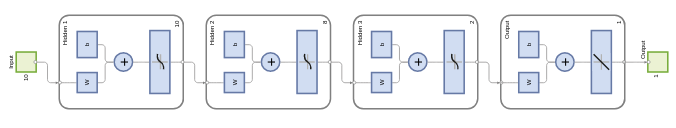
\includegraphics[width=\textwidth]{mlpmeanarch}
		\caption{ECG's mean estimation network
		architecture.}\label{fig:mlpmeanarch}
	\end{subfigure}
	\begin{subfigure}{\textwidth}
		\centering
		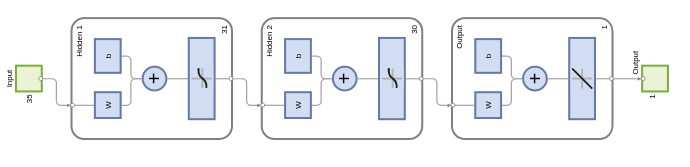
\includegraphics[width=\textwidth]{mlpstdarch}
		\caption{ECG's standard deviation estimation network
		architecture.}\label{fig:mlpstdarch}
	\end{subfigure}
	\caption{Graphical representation of the architectures selected by
	\code{bayesopt}.}\label{fig:mlparches}
\end{figure}

\section{MLPs training}\label{sec:mlptraining}

Script \texttt{mlptrain.m} performs the training of both networks using the
architectures selected in \secref{subsec:mlpbayesopt} and the training
algorithms and feature extraction methods selected in
\secref{subsec:mlphyperopt}.

\vfigref{fig:mlptrainperformance} shows the training performance plots for both
networks. 

\begin{figure}[htbp]
	\centering
	\begin{subfigure}{\textwidth}
		\centering
		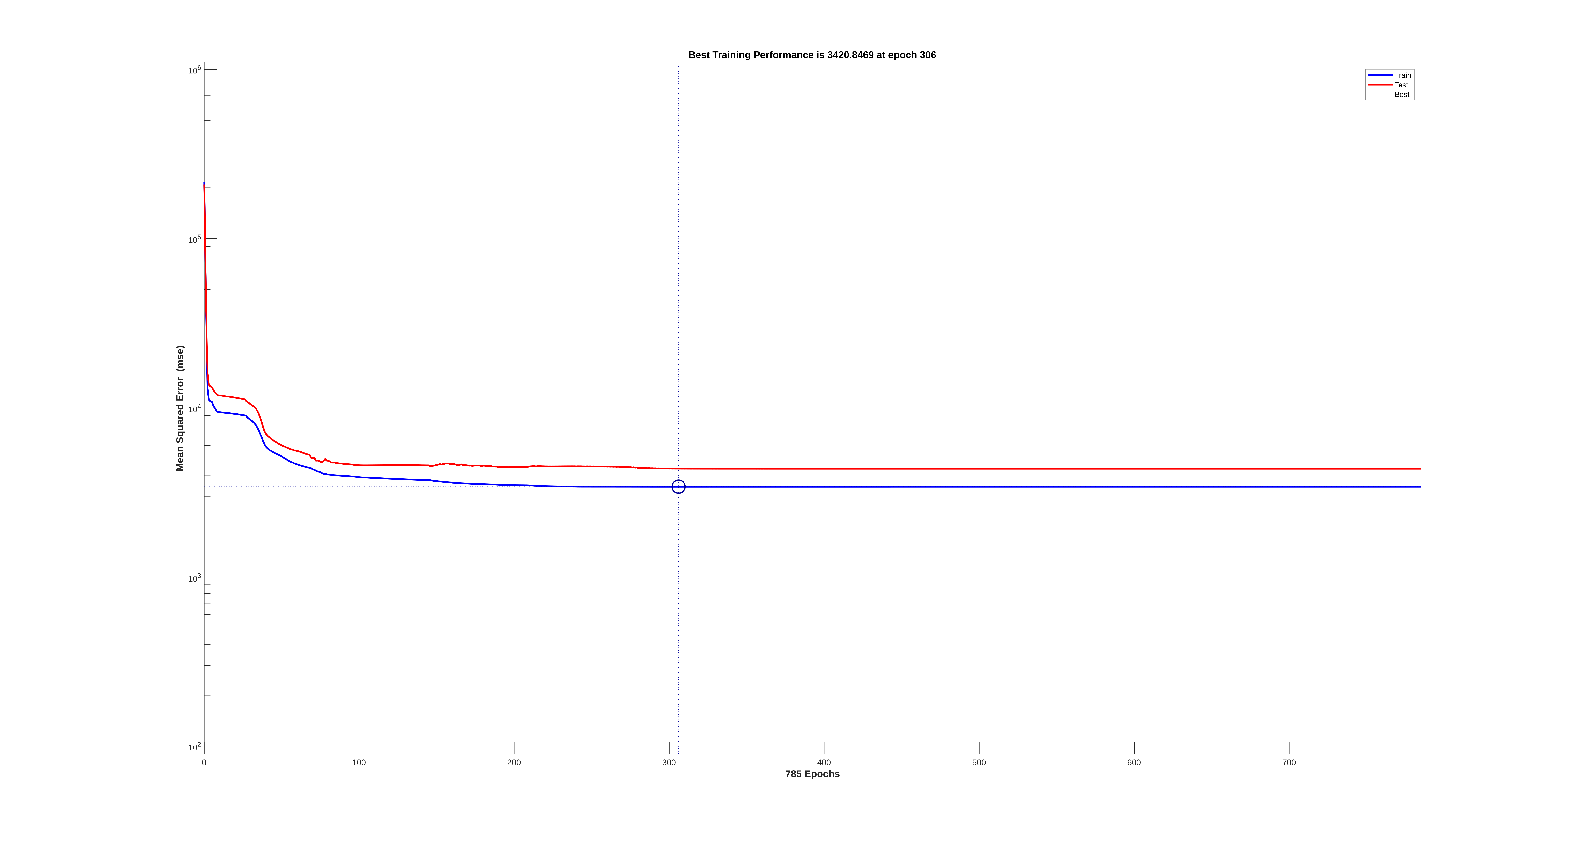
\includegraphics[width=\textwidth, trim=2.95cm 1.1cm 2cm 0.8cm,
		clip]{mlpmeantrainperformance}
		\caption{Training performance plot for the ECG's mean
		estimation network.}\label{fig:mlpmeantrainperformance}
	\end{subfigure}
	\begin{subfigure}{\textwidth}
		\centering
		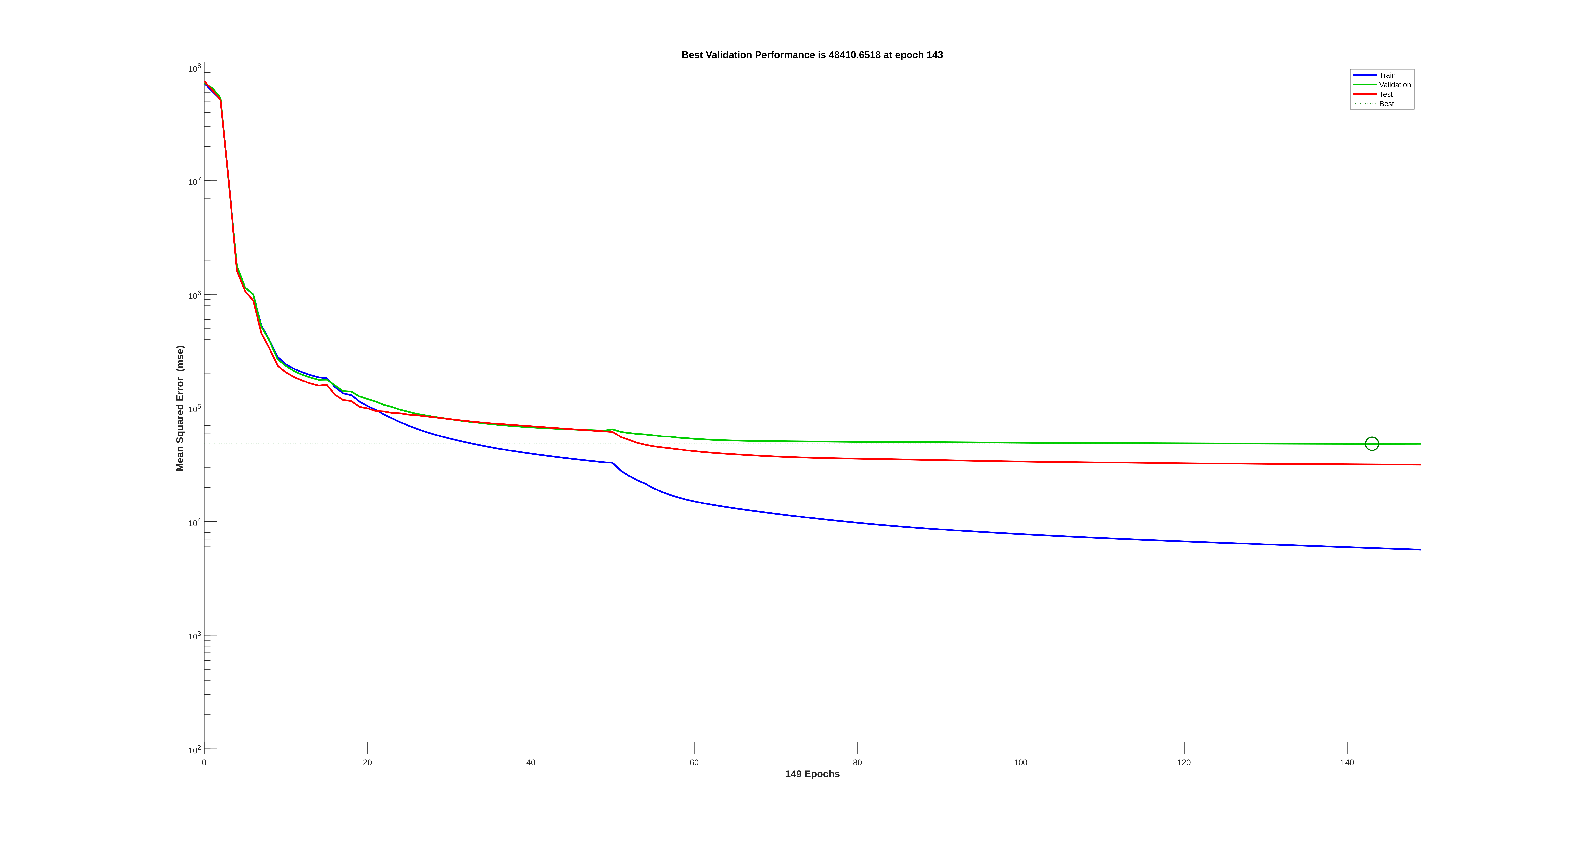
\includegraphics[width=\textwidth, trim=2.95cm 1.1cm 2cm 0.8cm,
		clip]{mlpstdtrainperformance}
		\caption{Training performance plot for the ECG's standard
		deviation estimation network.}\label{fig:mlpstdtrainperformance}
	\end{subfigure}
	\caption{Training performance plots for the two
	networks.}\label{fig:mlptrainperformance}
\end{figure}

\vfigref{fig:mlpstdregression} shows the regression plot for the ECG's standard
deviation estimation network. The network performs very well, with a
coefficient \(R = 0.99184\) for the test set and \(R = 0.99616\) for the entire
dataset.

\begin{figure}[htbp]
	\centering
	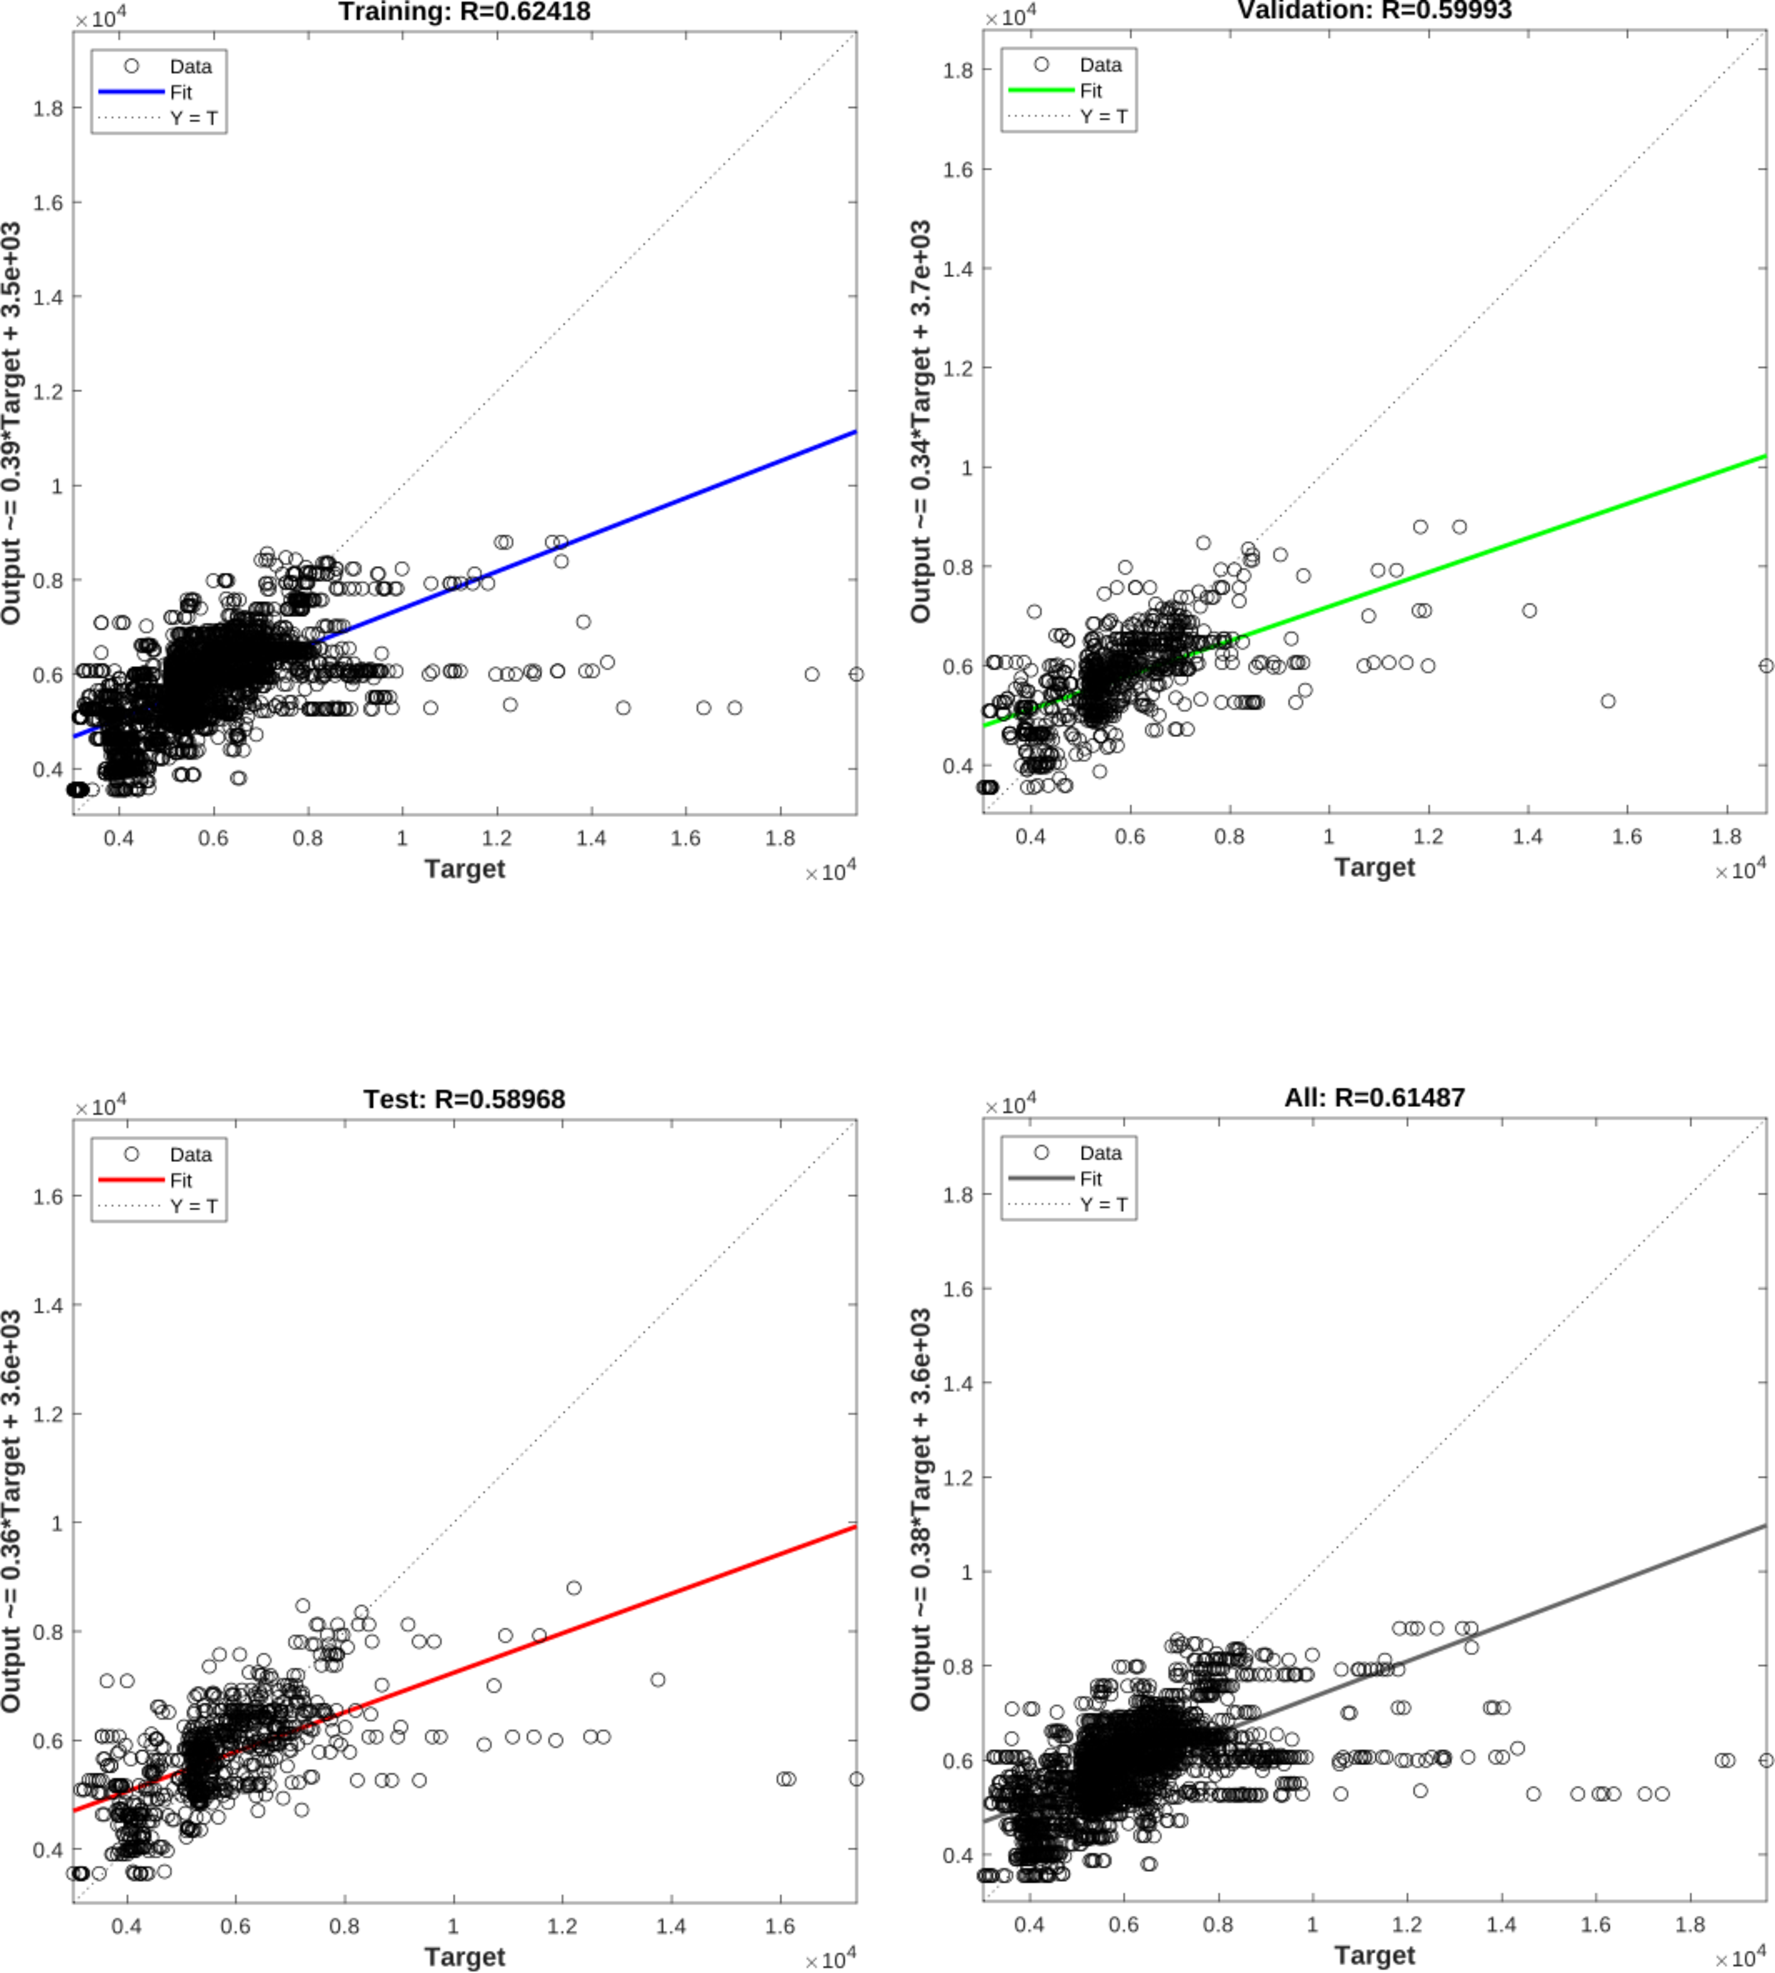
\includegraphics[width=\textwidth]{mlpstdregression}
	\caption{The regression plot for the ECG's standard deviation
	estimation network shows excellent
	results.}\label{fig:mlpstdregression}
\end{figure}

The ECG's mean estimation network performances are not so good (but still
valuable), as shown in \vfigref{fig:mlpmeanregression}: we have \(R = 0.85045\)
for the test set and \(R = 0.85761\) for the entire dataset. This latter
network will be the subject of \chref{ch:cnn}.

\begin{figure}[htbp]
	\centering
	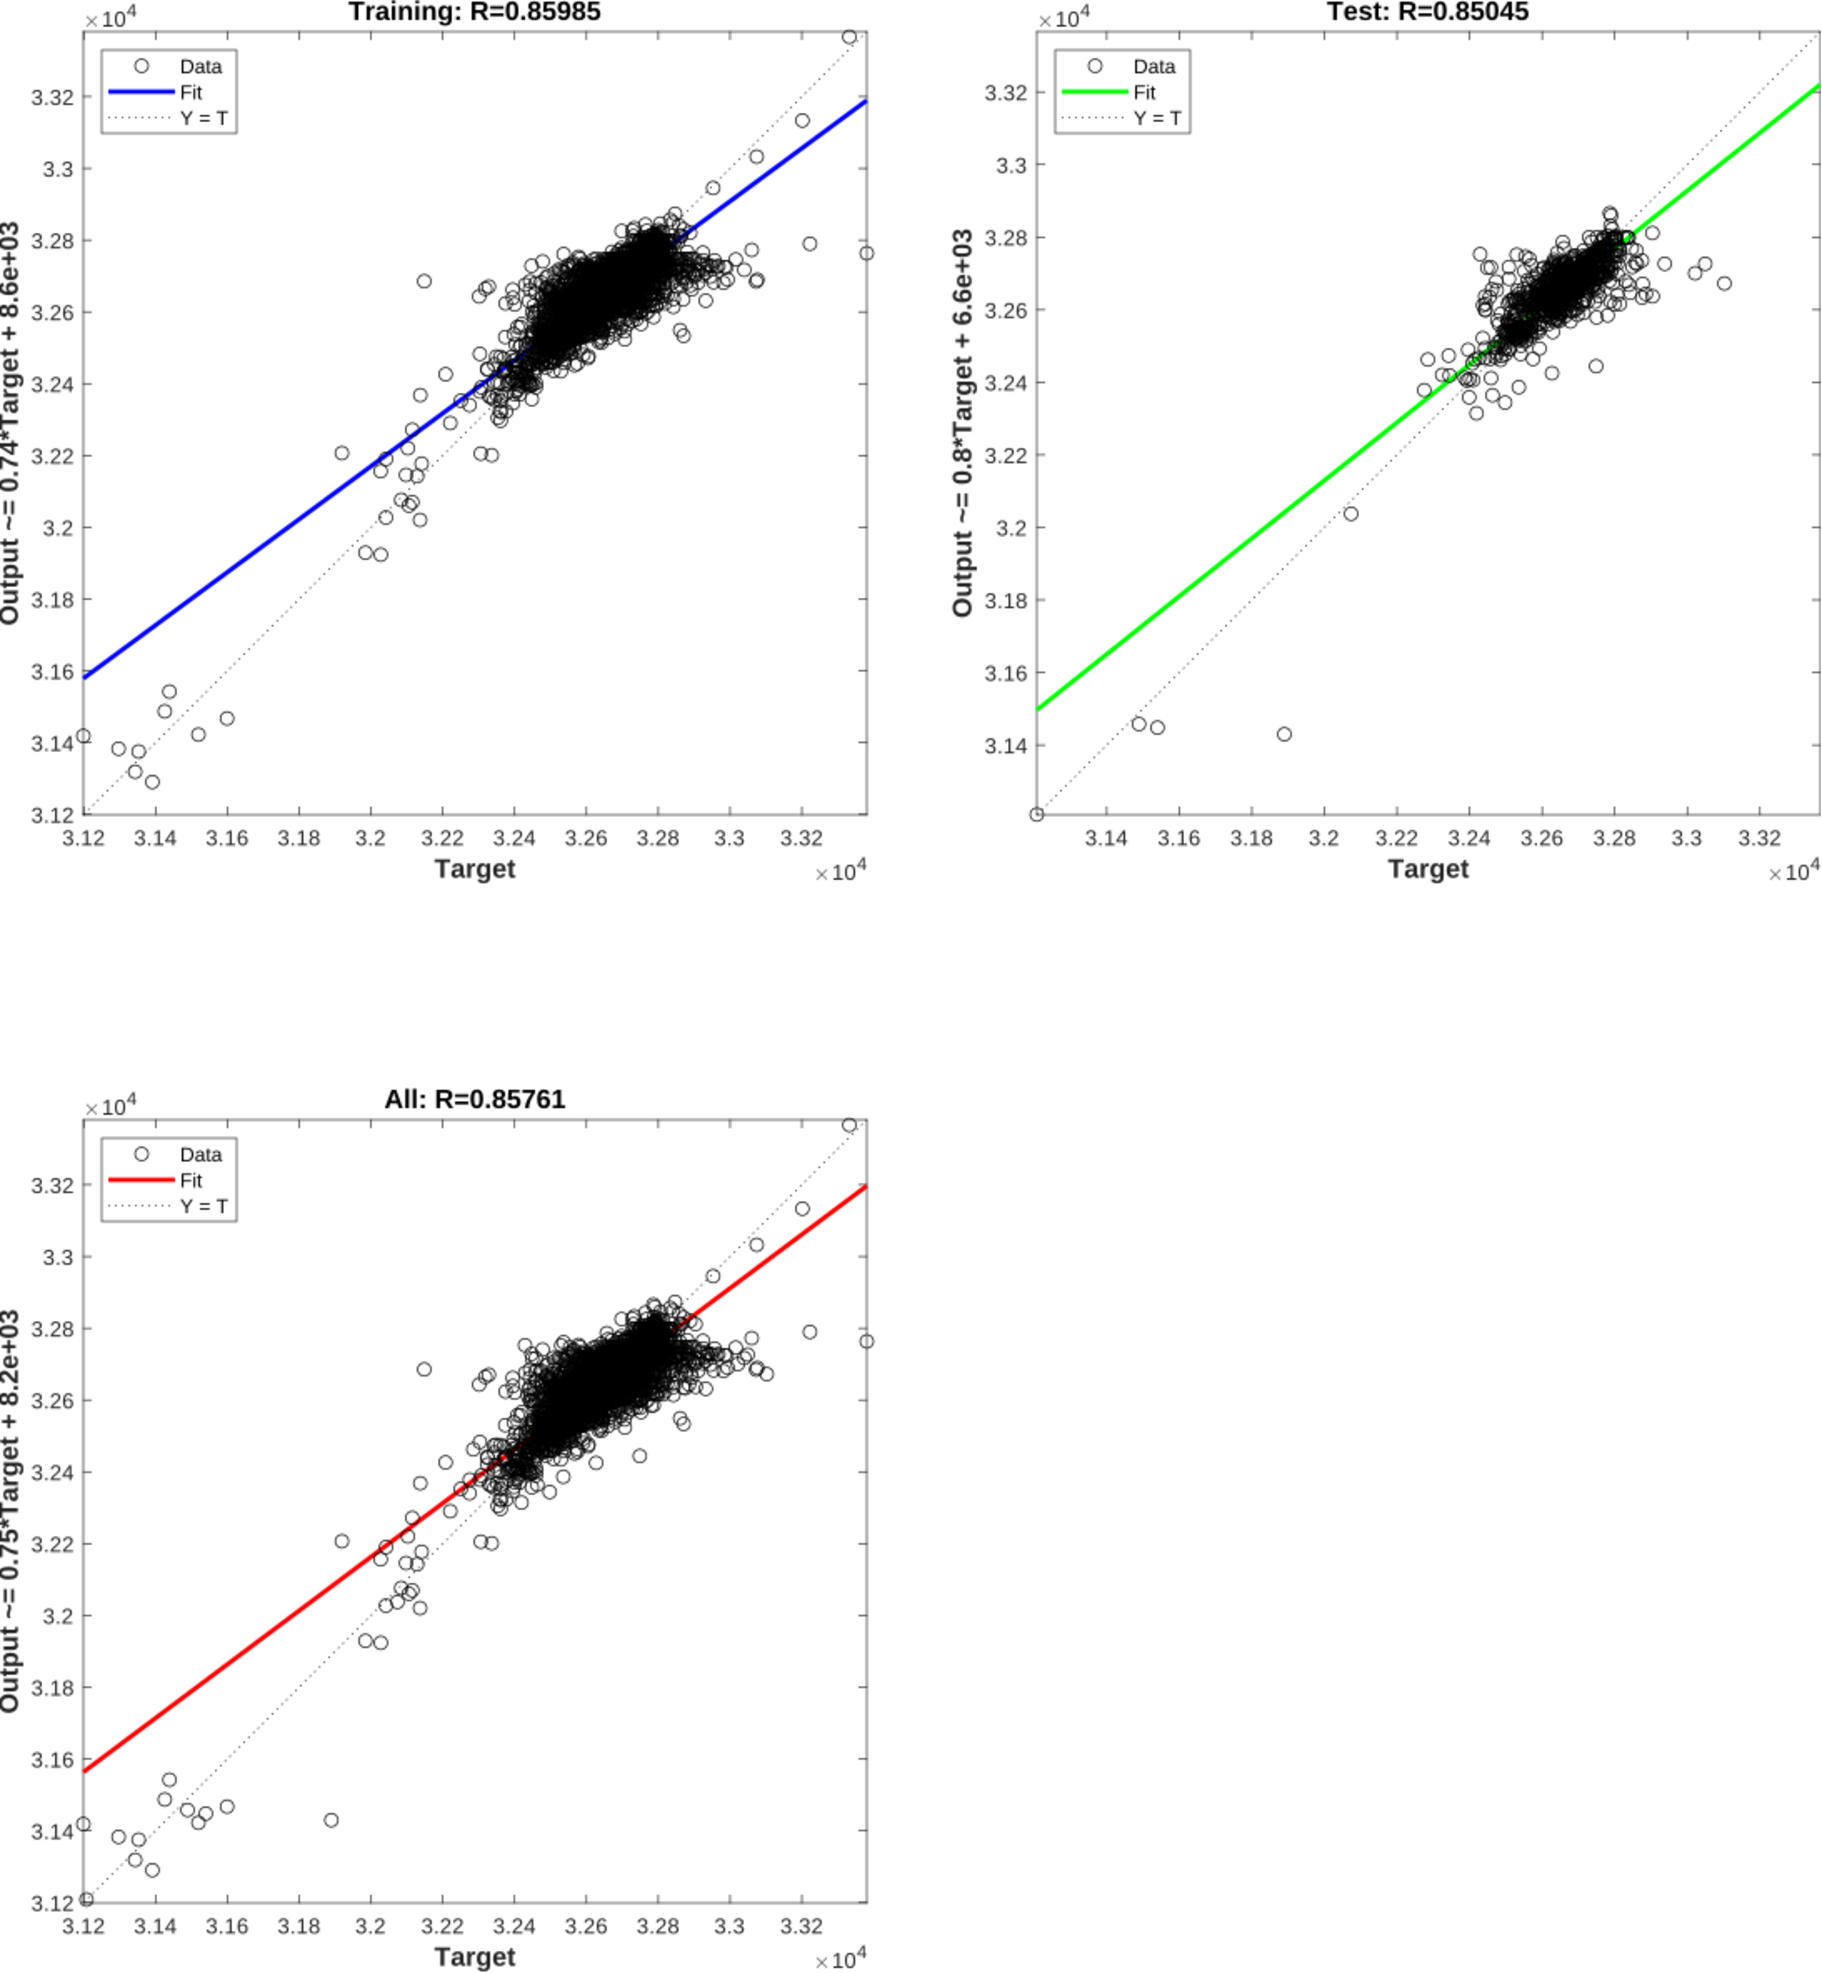
\includegraphics[width=\textwidth]{mlpmeanregression}
	\caption{The regression plot for the ECG's mean estimation network
	shows good, but not excellent, results.}\label{fig:mlpmeanregression}
\end{figure}

\vfigref{fig:mlperrorhists} shows the error histograms for both networks.

\begin{figure}[htbp]
	\centering
	\begin{subfigure}{\textwidth}
		\centering
		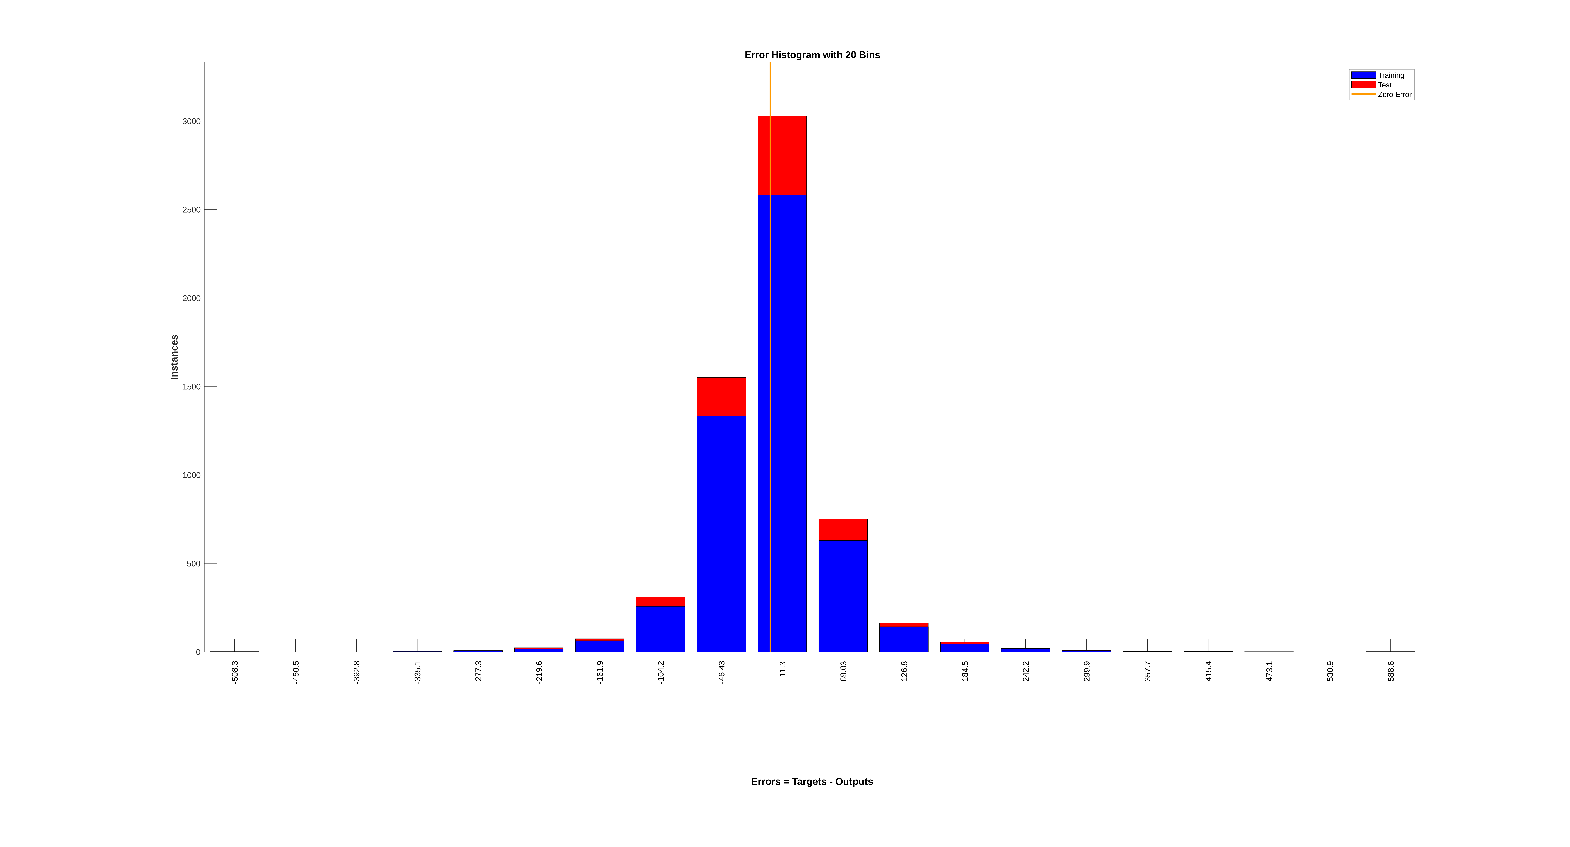
\includegraphics[width=\textwidth, trim=2.9cm 1cm 2cm 0.8cm,
		clip]{mlpmeanerrorhist}
		\caption{Error histogram for the ECG's mean estimation
		network.}\label{fig:mlpmeanerrorhist}
	\end{subfigure}
	\begin{subfigure}{\textwidth}
		\centering
		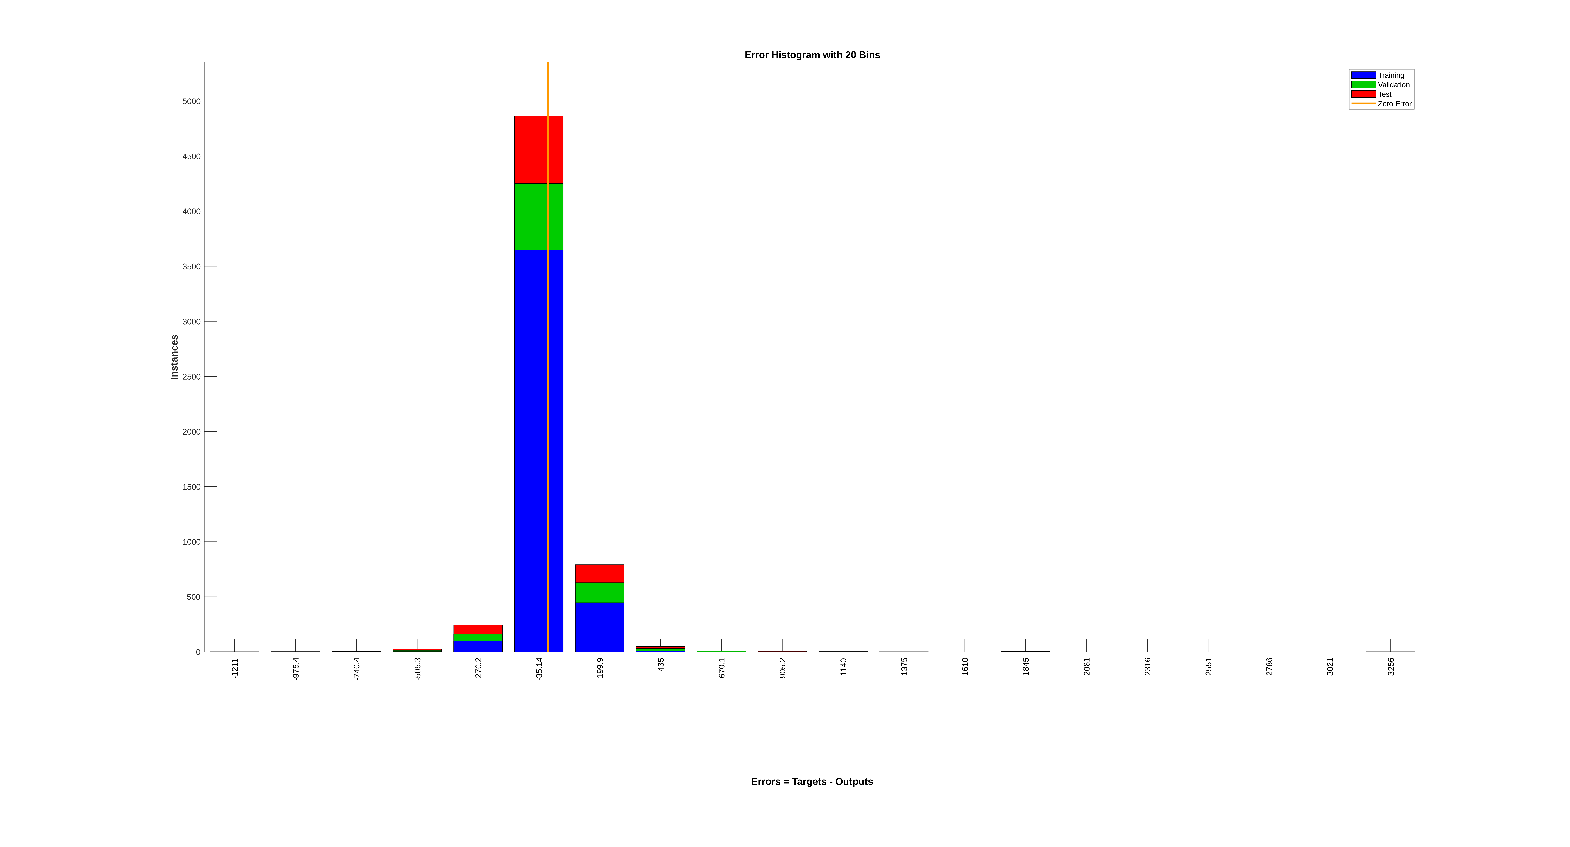
\includegraphics[width=\textwidth, trim=2.9cm 1cm 2cm 0.8cm,
		clip]{mlpstderrorhist}
		\caption{Error histogram for the ECG's standard deviation
		estimation network.}\label{fig:mlpstderrorhist}
	\end{subfigure}
	\caption{Error histograms for the two
	networks.}\label{fig:mlperrorhists}
\end{figure}


\chapter{Determining a person's activity}\label{ch:activity}

\chapter{Fuzzy inference system}\label{ch:fuzzy}

\chapter{ECG mean using a Convolutional Neural Network}\label{ch:cnn}

\chapter{ECG prediction using a Recurrent Neural Network}\label{ch:rnn}


\end{document}
